% !TeX encoding = UTF-8
% Lecture file created by newnote
% Class: Models of Theoretical Physics
% Professor: Azaele Sandro
% Date: 2025-10-10
\lecture{15}{Laplace method continued}{2025-10-10}
\pagelayout{margin}
% --- Start writing here ---

\section{Laplace method continued}
\subsection*{The Laplace method}
In several situations we wish to evaluate complicated integrals which have a
form
\begin{DispWithArrows}[displaystyle, format=c]
  I(\lambda)=\int_{x_{1}}^{x_{2}} d x g(x) e^{\lambda f(x)} \quad \lambda \in \mathbb{R}
\end{DispWithArrows}
where $g$ and $f$ are continuous and differentiable functions. Although
$I(\lambda)$ cannot be calculated for any arbitrary $\lambda$, it happens that
it can be well approximated (under appropriate conditions) as
$\lambda \rightarrow \infty$.
The core idea of Laplace's method is that the major contribution to the
integral in (21) as $\lambda \rightarrow \infty$ comes from the neighborhood of
the point in $\left[x_{1}, x_{2}\right]$ where $f(x)$ gets its maximum value,
which we call $x_{0}$.
\begin{figure}[H]
  \centering
  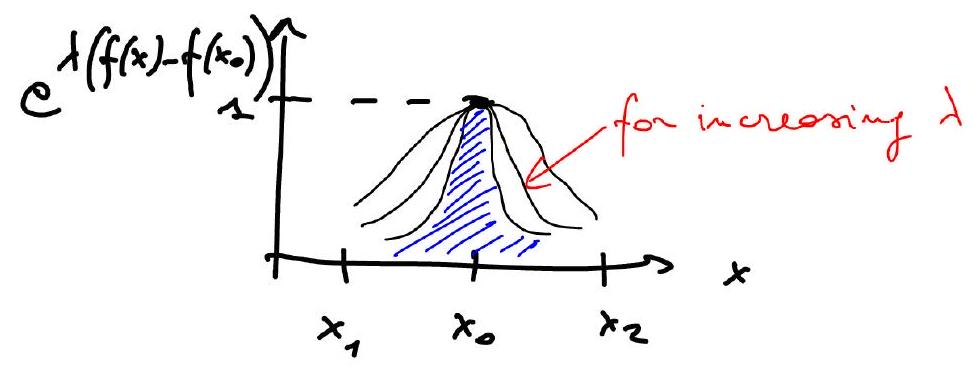
\includegraphics[width=\textwidth]{graphics/2025_10_19_6d9f59a2c3b97d481c52g-1}
\end{figure}
There are essentially three cases:
\begin{enumerate}
  \item $x_{0}$ is an interior maximum, $x_{1}<x_{0}<x_{2}$ and
    $f^{\prime}\left(x_{0}\right)=0$. We assume that
    $f^{\prime \prime}\left(x_{0}\right)<0$ (actually if
    $f^{\prime}\left(x_{0}\right)=f^{\prime \prime}\left(x_{0}\right)=f^{\prime \prime \prime}\left(x_{0}\right)=0$
    but $f^{(iv)}\left(x_{0}\right)<0$ we can apply very similar ideas and the
    calculations are not more difficult). Also $g\left(x_{0}\right) \neq 0$ and
    it is finite.
\end{enumerate}
As we expect that the dominant contributions comes from the neighborhood of
$x_{0}$ and
$f(x)=f\left(x_{0}\right)+\frac{\left(x-x_{0}\right)^{2}}{2} f^{\prime \prime}\left(x_{0}\right) +O\left(\left|x-x_{0}\right|^{3}\right)$
as $x \rightarrow x_{0}$, we obtain
\begin{DispWithArrows}[displaystyle, format=c]
  I(\lambda) \cong \int_{x_{1}}^{x_{2}} g(x) e^{\lambda\left(f\left(x_{0}\right)+\frac{\left(x-x_{0}\right)^{2}}{2} f^{\prime \prime}\left(x_{0}\right)\right)} d x \simeq g\left(x_{0}\right) e^{\lambda f\left(x_{0}\right)} \int_{x_{1}}^{x_{2}} e^{-\lambda \frac{\left|f^{\prime \prime}\left(x_{0}\right)\right|}{2}\left(x-x_{0}\right)^{2}} d x
\end{DispWithArrows}
We change var.
$s=\left(x-x_{0}\right) \sqrt{\frac{\left|f^{\prime \prime}\left(x_{0}\right)\right|}{2} \lambda}$
so
\begin{DispWithArrows}[displaystyle, format=c]
  I(\lambda) \simeq g\left(x_{0}\right) e^{\lambda f\left(x_{0}\right)} \sqrt{\frac{2}{\lambda\left|f^{\prime \prime}\left(x_{0}\right)\right|}} \int_{\left(x_{1}-x_{0}\right) \sqrt{\frac{\left|f^{\prime \prime}\left(x_{0}\right)\right| \lambda}{2}}}^{\left(x_{2}-x_{0}\right) \sqrt{\frac{\left|f^{\prime \prime}\left(x_{0}\right)\right| \lambda}{2}}} e^{-s^{2}} d s
\end{DispWithArrows}
as
$\lambda \rightarrow \infty \rightarrow \int_{-\infty}^{+\infty} e^{-s^{2}} d s=\sqrt{\pi}$
\begin{DispWithArrows}[displaystyle, format=c]
  I(\lambda) \simeq g\left(x_{0}\right) e^{\lambda f\left(x_{0}\right)} \sqrt{\frac{2 \pi}{\lambda\left|f^{\prime \prime}\left(x_{0}\right)\right|}} \quad \text { as } \lambda \rightarrow+\infty \text { (leading order)}
\end{DispWithArrows}
one should prove that this is the leading order (we did not).

Exercise: show that the next to leading order of $I(\lambda)$ in eq. (22) is
given by
\begin{DispWithArrows}[displaystyle, format=c]
  I(\lambda)=e^{\lambda f\left(x_{0}\right)} \sqrt{\frac{2 \pi}{\lambda\left|f^{\prime \prime}\left(x_{0}\right)\right|}}\left(g\left(x_{0}\right)+\frac{c}{\lambda}\right) \quad \text { as } \lambda \rightarrow \infty
\end{DispWithArrows}
where $c$ is a constant that depends on the derivatives of $f$ up to
$4^{\text {th }}$ order (at $x=x_{0}$) and on $g\left(x_{0}\right)$ and
$g^{\prime}\left(x_{0}\right)$.
\begin{enumerate}
  \setcounter{enumi}{1}
  \item $x_{0}=x_{1}$ or $x_{0}=x_{2}$ ($x_{0}$ is a flat endpoint) and
    $f^{\prime}\left(x_{0}\right)=0$.
    \begin{figure}[H]
      \centering
      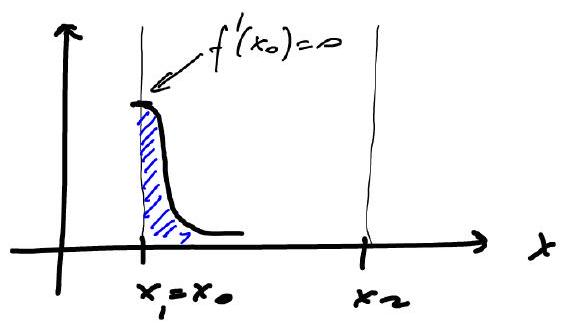
\includegraphics[width=0.5\textwidth]{graphics/2025_10_19_6d9f59a2c3b97d481c52g-3}
    \end{figure}
    It is easy to show that the leading order formula is
    \begin{DispWithArrows}[displaystyle, format=c]
      I(\lambda) \simeq g\left(x_{0}\right) e^{\lambda f\left(x_{0}\right)} \sqrt{\frac{\pi}{2 \lambda\left|f^{\prime \prime}\left(x_{0}\right)\right|}}
    \end{DispWithArrows}
\end{enumerate}
\subsection*{Example}
The modified Bessel function of second kind is a special function that occurs
in many applications. It is given by
\begin{DispWithArrows}[displaystyle, format=c]
  K_{\nu}(x)=\int_{0}^{\infty} e^{-x \cosh t} \cosh (\nu t) d t, x>0
\end{DispWithArrows}
we wish to estimate $K_{\nu}(x)$ as $x \rightarrow+\infty$ for fixed $\nu$.
Since $\cosh^{\prime}(t)=\sinh (t)>0$ for $t>0$, the max of $e^{-x \cosh t}$ as
a function of $t(x>0)$ occurs at $t=0$, with zero derivative.

So we can apply eq. (23) ($\cosh t \simeq 1+\frac{t^{2}}{2}+\cdots$)
$f(t)=-\cosh t$
\begin{DispWithArrows}[displaystyle, format=c]
  K_{\nu}(x) \simeq e^{-x} \sqrt{\frac{\pi}{2x}}
\end{DispWithArrows}
as $x \rightarrow \infty$ at leading order.

Notice that it does not depend on $\nu$!
Exercise: show that
\begin{DispWithArrows}[displaystyle, format=c]
  K_{\nu}(x)=\sqrt{\frac{\pi}{2x}} e^{-x}\left(1+\frac{c(\nu)}{x}+\cdots\right)
\end{DispWithArrows}
and $c(\nu)=\frac{4 \nu^{2}-1}{8}$.
\begin{enumerate}
  \setcounter{enumi}{2}
  \item $x_{0}=x_{1}$ or $x_{0}=x_{2}$ ($x_{0}$ is an endpoint) but
    $f^{\prime}\left(x_{0}\right) \neq 0$. Without loss of generality we take
    $x_{0}=x_{1}$ and $f^{\prime}\left(x_{0}\right)<0$.
    \begin{figure}[H]
      \centering
      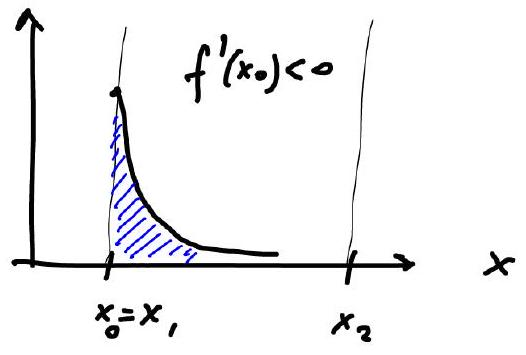
\includegraphics[width=0.5\textwidth]{graphics/2025_10_19_6d9f59a2c3b97d481c52g-4}
    \end{Figure}
    In this case we get
    $f(x)=f\left(x_{0}\right)+\left(x-x_{0}\right) f^{\prime}\left(x_{0}\right)+\cdots$
    hence
    \begin{DispWithArrows}[displaystyle, format=ll]
      \begin{aligned}
        I(\lambda) & \cong \int_{x_{1}=x_{0}}^{x_{2}} g(x) e^{\lambda\left[f\left(x_{0}\right)+\left(x-x_{0}\right) f^{\prime}\left(x_{0}\right) \right]} d x \\
        & =g\left(x_{0}\right) e^{\lambda f\left(x_{0}\right)} \int_{x_{0}}^{x_{2}} e^{\lambda\left[\left(x-x_{0}\right) f^{\prime}\left(x_{0}\right) \right]} d x \\
        & =g\left(x_{0}\right) e^{\lambda f\left(x_{0}\right)} \int_{0}^{x_{2}-x_{0}} e^{\lambda f^{\prime}\left(x_{0}\right) s} d s=\frac{g\left(x_{0}\right) e^{\lambda f\left(x_{0}\right)}}{\lambda f^{\prime}\left(x_{0}\right)}\left[e^{\lambda s f^{\prime}\left(x_{0}\right)} \right]_{0}^{x_{2}-x_{1}}
      \end{aligned}
    \end{DispWithArrows}
as $\lambda \rightarrow \infty$ and $f^{\prime}\left(x_{0}\right)<0$ we get
    \begin{DispWithArrows}[displaystyle, format=c]
      I(\lambda) \cong g\left(x_{1}\right) \frac{e^{\lambda f\left(x_{1}\right)}}{\lambda\left|f^{\prime}\left(x_{1}\right)\right|} \quad \text { as } \lambda \rightarrow \infty
    \end{DispWithArrows}
\end{enumerate}
\subsection*{Example:}
Obtain the leading order approximation of
\begin{DispWithArrows}[displaystyle, format=c]
  I(\lambda)=\int_{0}^{1} x^{m} e^{\lambda\[3 x^{2}+2 x^{3}\]} d x \quad \text { as } \lambda \rightarrow+\infty
\end{DispWithArrows}
\begin{figure}[H]
  \centering
  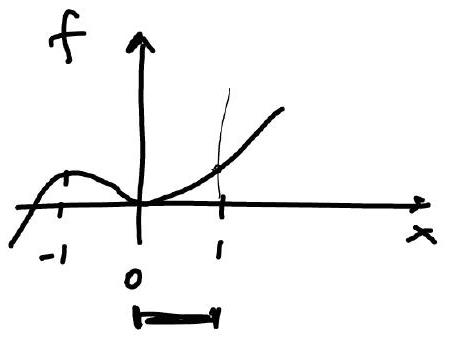
\includegraphics[width=0.5\textwidth]{graphics/2025_10_19_6d9f59a2c3b97d481c52g-5}
\end{figure}
The max is at $x=1, f(1)=5, f^{\prime}(1)=12, g(1)=1$. We can apply eq. (24)
\begin{DispWithArrows}[displaystyle, format=c]
  I(\lambda) \simeq \frac{e^{5\lambda}}{12 \lambda}
\end{DispWithArrows}
\subsection*{Exercise:}
Calculate the leading order approx. when the integral is
\begin{DispWithArrows}[displaystyle, format=c]
  \int_{-1}^{0} \cdots=? \quad \int_{-2}^{0} \cdots=?
\end{DispWithArrows}
\subsection*{Stirling formula}
We want to estimate how fast $N!$ goes to infinity as $N \rightarrow \infty$. We
will apply the Laplace's method to the gamma function:
\begin{DispWithArrows}[displaystyle, format=c]
  \Gamma(\lambda)=\int_{0}^{\infty} x^{\lambda-1} e^{-x} d x \quad \lambda>0
\end{DispWithArrows}
Exercise: Show that $\Gamma(\lambda+1)=\lambda \Gamma(\lambda)$ hence
$\lambda!=\Gamma(\lambda+1)$ which generalize the factorial to complex numbers.

Let's consider $\Gamma(\lambda+1)=\int_{0}^{\infty} x^{\lambda} e^{-x} d x$. If
we write this as $\int_{0}^{\infty} e^{-x} e^{\lambda \ln x} d x$ we cannot apply
Laplace's method. It is more beneficial to consider the max of the function
$f(x)=-x+\lambda \ln x$ and set $g(x)=1$. The max occurs at $x=\lambda$ which
suggests a change of var: $x=\lambda t$ (so the max is now fixed w.r.t. t). We
get
\begin{DispWithArrows}[displaystyle, format=c]
  \Gamma(\lambda+1)=\int_{0}^{\infty} x^{\lambda} e^{-x} d x=\lambda^{\lambda+1} \int_{0}^{\infty} t^{\lambda} e^{-\lambda t} d t
\end{DispWithArrows}
$t^{\lambda} e^{-\lambda t}=e^{\lambda(\ln t-t)} \quad h(t)=\ln t-t, \quad h^{\prime}(1)=0, h^{\prime \prime}(1)=-1$.
In this way we can apply eq. (22) with $g(t)=1 \quad\left(t_{0}=1\right)$.
\begin{DispWithArrows}[displaystyle, format=c]
  \Gamma(\lambda+1)=\lambda!\simeq \lambda^{\lambda+1} e^{-\lambda} \sqrt{\frac{2 \pi}{\lambda}} \quad \text { as } \lambda \rightarrow \infty
\end{DispWithArrows}
Exercise: Show that at leading order
\begin{DispWithArrows}[displaystyle, format=c]
  \int_{0}^{\infty} e^{-\lambda t} e^{-\frac{1}{t}} d t \cong \frac{\sqrt{\pi} e^{-2 \sqrt{\lambda}}}{\lambda^{3 / 4}} \quad \text { as } \lambda \rightarrow \infty
\end{DispWithArrows}
\subsection*{Example:}
Let's consider the class of integrals:
\begin{DispWithArrows}[displaystyle, format=c]
  I_{m}(x)=\int_{0}^{\infty} t^{m} e^{-\frac{t^{2}}{2}-\frac{x}{t}} d t \quad x>0 .
\end{DispWithArrows}
We calculate $I_m(x)$ for large $x$ and fixed m.
$ \frac{t^{2}}{2}+ \frac{x}{t}$ has a movable min at $ \frac{d}{d t}
\left( \frac{t^{2}}{2}+\frac{x}{t}\right)=0, \bar{t}=x^{1 / 3}$. So we introduce
the new variable $\tau$:
\begin{DispWithArrows}[displaystyle, format=c]
  t=x^{1 / 3} \tau
\end{DispWithArrows}
So
\begin{DispWithArrows}[displaystyle, format=c]
  I_{m}(x)=x^{\frac{m+1}{3}} \int_{0}^{\infty} \tau^{m} e^{-x^{2 / 3}\left(\frac{\tau^{2}}{2}+\frac{1}{\tau}\right)} d \tau
\end{DispWithArrows}
The min of the exponent occurs at $\tau=1$ (interior) so we can apply eq. (22):
\begin{DispWithArrows}[displaystyle, format=ll]
  \begin{aligned}
    I_{m}(x) & =x^{\frac{m+1}{3}} e^{-\frac{3}{2} x^{2 / 3}} \sqrt{\frac{2 \pi}{x^{2 / 3} \cdot 3}} \\
    &=x^{m / 3} e^{-\frac{3}{2} x^{2 / 3}} \sqrt{\frac{2 \pi}{3}}
  \end{aligned}
\end{DispWithArrows}
as $x \rightarrow \infty$. leading order, fixed $m$

\subsection*{Exercises:}
\begin{DispWithArrows}[displaystyle, format=ll]
  \begin{aligned}
    & \int_{-2}^{0} e^{t} e^{\lambda\[3 t^{2}+2 t^{3}\]} d t \simeq e^{\lambda-1} \sqrt{\frac{\pi}{3 \lambda}} \\
    & \int_{0}^{1} e^{t} e^{\lambda\[3 t^{2}+2 t^{3}\]} d t \simeq \frac{e^{5\lambda+1}}{12 \lambda} \\
    & \int_{0}^{1} \sqrt{1+t} e^{\lambda\[2 t-t^{2}\]} d t \simeq e^{\lambda} \sqrt{\frac{\pi}{2 \lambda}} \\
    & \int_{-1}^{2} e^{\lambda\[t^{3}-1\]}\left(1+t^{2}\right) d t \simeq \frac{5 e^{7\lambda}}{11 \lambda}
  \end{aligned}
\end{DispWithArrows}
Question: Let's assume that $f(x)$ behaves like in the fig:
\begin{figure}[H]
  \centering
  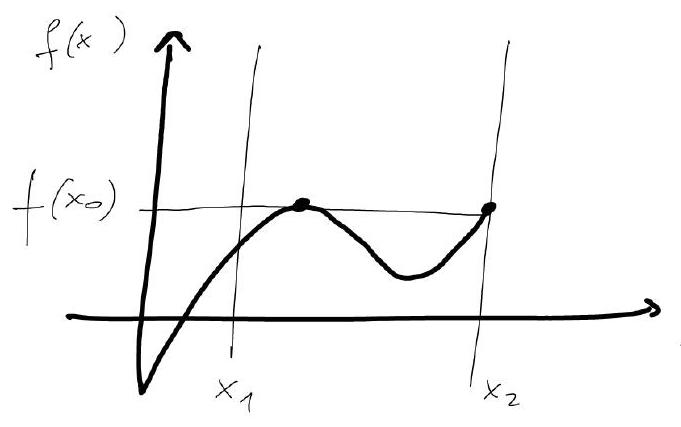
\includegraphics[width=0.5\textwidth]{graphics/2025_10_19_6d9f59a2c3b97d481c52g-8}
\end{figure}
Where does the leading order come from?
